\section{Annotation Procedure}
\label{sec:annotation}
This section describes how an annotator annotates a Turkish sentence.

An annotator selects a sentence from a treebank, which has previously uploaded sentences coming from a CoNLL-U formatted file.
They fill the cells of the annotation table's fields.
During the annotation, an annotator can make use of dependency graphs, error cards and the search functionality.
Dependency graphs are visual cues for how an annotation is going, using HEADs and DEPRELs.
They can choose 3 different graphs one at a time or select to hide.
Different graphs show the same information with a horizontal or vertical tree.
Errors are helpful reminders, coming from a validation script found on the UD repository.
They can use the search functionality to search for previous annotations by other annotators or themselves, using various fields (text, FEATS, etc.) for the query.
By checking similar annotations, an annotator can ensure consistency and don't lose focus by trying manual methods for the same information.
When an annotation is done, they select the annotation to be "Complete".

%\begin{figure}[tbh]
%	\centering
%	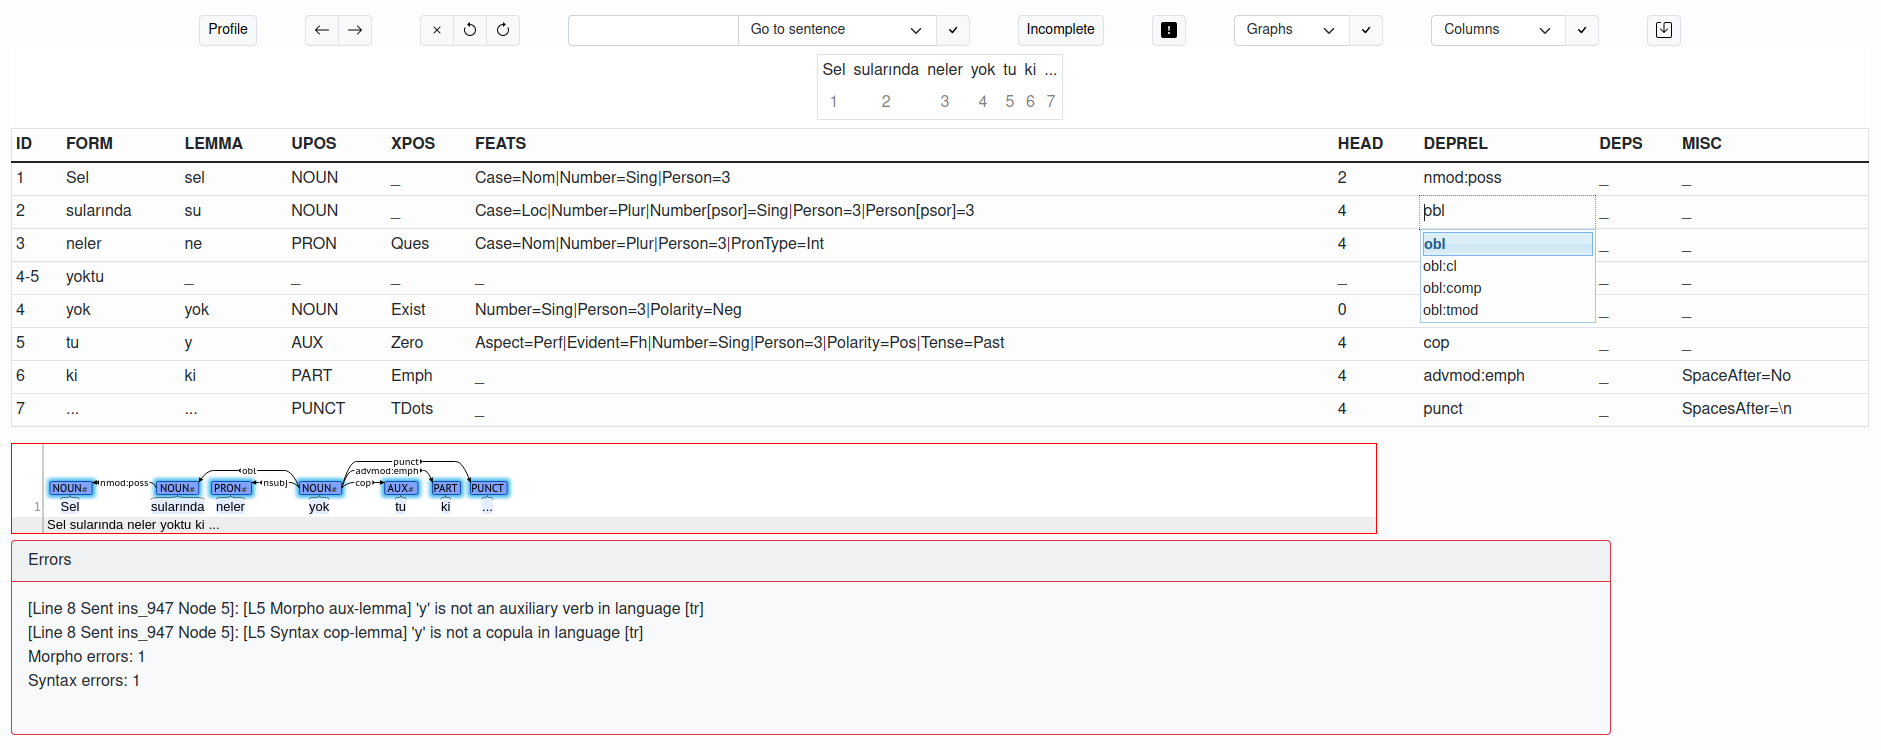
\includegraphics[width=0.6\textwidth]{1.png}
%	\caption{Once upon a time, kids could not wait to get their hands on these booklets obtained from Dandy chewing gum.}
%	\label{fig:demo-fig}
%\end{figure}

